\documentclass{article}
\usepackage[utf8]{inputenc}

\usepackage{authblk}
\usepackage{multicol}
%\usepackage{natbib}
\usepackage{graphicx}
\usepackage{abstract}
\usepackage{float}
\usepackage[english]{babel}
\usepackage{amsmath}
\usepackage{subfigure}
\usepackage{alltt}
\usepackage{url}
\usepackage{multirow}
\usepackage[margin=4cm]{geometry}



\title{Human Connectome: Visualization Techniques and Methodologies}
\author{Giorgio Conte}
%\date{December, $11^{th}$ 2014}
\affil{Creative Coding Research Group\\ Department of Computer Science\\University of Illinois at Chicago}



\begin{document}

\maketitle
\begin{abstract}
\end{abstract}

\begin{multicols}{2}
\raggedcolumns

\section{Introduction}

Being able to deeply understand how the brain is working is one of the main challenges in the last years among neuroscientists. With the advent and the refinement of new technologies like fMRi and diffusion MRI, doctors are able to collect and derive data about how the regions of the brain are connected. Very frequently the map of neural connections of the brain is addressed as CONNECTOME.
Visualizing these data in an effective way allows people to navigate and explore all the wired connections that are in the brain. Moreover, thanks to this kind of visualizations is possible to understand better what differences there are between healthy subjects and other people who suffer from a wide range of neuropsychiatric illnesses like bipolar, body dysmorphic disorder, Alzheimer?s disease and late-life depression. 
Many visualization tools have been proposed in the academic literature, however the vast majority of them perform 2D visualizations. However, since this research field is quite novel, there is still room for improvement.
The aim of this work is to report and survey the visualizations tools already present in the academic literature as well as to introduce which the new trends for the near future are.\\
The paper is structured as follows. In section there is a more detailed introduction about the human connectome. Then, a detailed list of common tasks follows, while in section NUMERO I describe accurately the most interesting tool. In section ... to be continued.
%-------------------------------------------------------------------------
\section{Domain}
Human Connectome has been always considered by neuroscientists a very interesting and challenging topic. However, it is only in the last few ten years, when more powerful and more accurate technologies took place firmly in the research area, that more detailed studies have been conducted. Moreover, thanks to new technologies it is now possible to get data from living human subject, that is why they are also addressed as \textit{in vivo} techniques. In fact, thanks to very advanced procedure and algorithms, experts can collect data about the functional and structural connectivity of the brain \textit{in vivo}. As it it reported by Behrend and Sporns in \cite{humanConnectomics}, among all the methodologies there are two main approaches to collect data and they rely on very different principles. On the one hand there is \textit{diffusion tractography} that infers the path of neuronal axons as they go across the brain's white matter by the measure of the water molecules in and around the axons, on the other hand \textit{resting-state functional MRI} measures the fluctuation in the \textit{blood-oxigenation-level-dependent} signal in brain's grey matter regions. More in details, fMRI does not measure directly the connections, but its aim is to find patterns and it expresses connectivity as statical dependencies in the grey matter activity. Although the meanings of the dataset collected are quite different, what the neuroscientists can obtain is a parcellation of the brain into smaller subregions as well as the strength of the connections, whether structural or functional, that link brain's regions. So, going to an higher level of abstraction, the entire Connectome could be seen as a very dense and highly connected graph, where nodes correspond to neural elements (brain's regions) and edges define their interconnections. Rubinov and Sporns in \cite{complexNetworkMeasures} were the first authors that consider the human connectome as a graph and in turns they described and applied many graph-based metrics to the connectome. Since, as aforementioned, the networks obtained are highly dense, the main challenge should be addressed is that task of "creating intuitive, informative and candid images" as it is highlighted by Margulies et al. in \cite{visualizingHumanConnectome}

\section{Main Tasks}
One of the worse mistake that can be done when designing a visual analytics tool is the willingness of addressing a spread set of tasks. So that is why is important to clearly understand and then state what the main tasks in a given research area are. This activity it is not as simple as it might seem at a first glance. So, in this section I am trying to describe as much clear as possible the main goals that neuroscientist would achieve using a human connectome visualization tool.\\
Due to the high complexity of the brain network, \textit{exploration} is the the most important task. Although some readers may argue that the exploration task is too simple, pretty obvious and too general, in my opinion, it is not so. In fact, especially when the field is quite novel and with many uncleared aspects, as it is the one we are talking about, it is extremely relevant to allow to user a \textit{visualization flexibility}. Flexibility should be achieved in terms of level of abstraction, perspective and data that can be visualized. \\
\textit{Comparison} is the other task that should be achieved by a visual analytics tool. For example, neuroscientists are usually interested in comparing healthy and diseased subjects, so that it is possible to understand if there are different connectivity patterns in the brain network, which connections are missing and which are still active. For example, in studies like the one proposed by Bassett et al. in \cite{hierarchicalOrganization} shows there are topological and connectivity differences in schizophrenic patients with respect to healthy subjects. So, having an easy-to-use visualization tool could accelerate this process and could hopefully allow more interesting discoveries.

\section{Survey}
\begin{figure*}[ht]
\centering
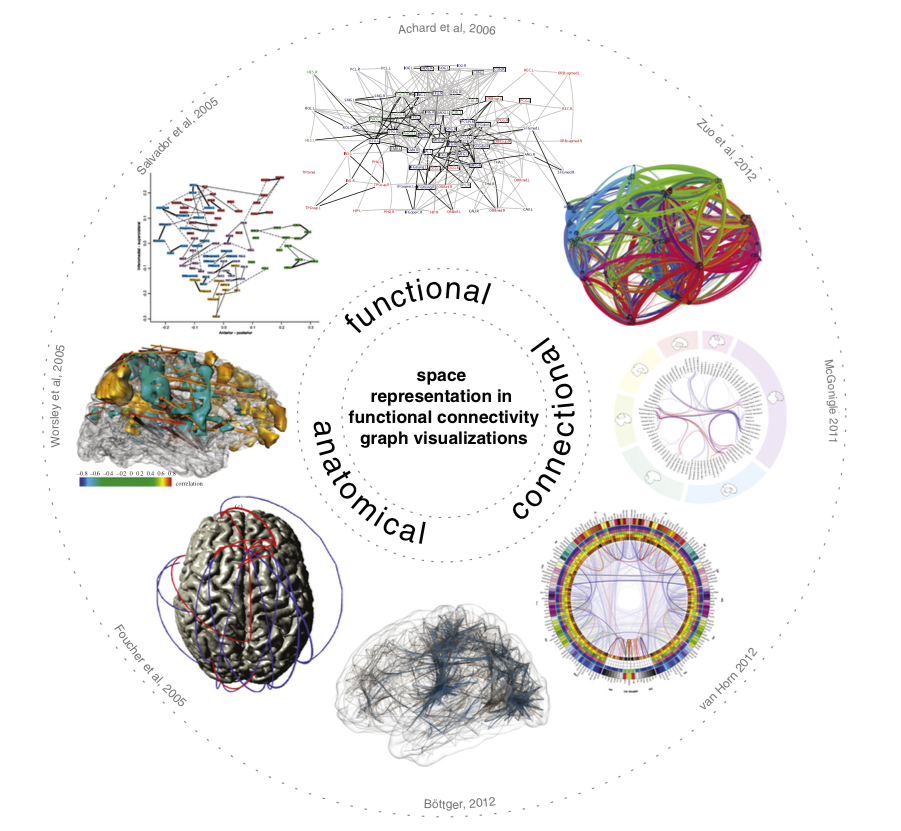
\includegraphics[width = 1.8\columnwidth]{taxonomy}
\caption{Images taken from \cite{visualizingHumanConnectome}}
\label{fig:taxonomy}
\end{figure*}

Many visualization tools have been presented in the academic literature, but ,before describing more in details, I would like to report the interesting taxonomy presented in \cite{visualizingHumanConnectome} by Margulies et al. In fact, they identified three main categories of visualization methodologies for the human Connectome and they are as follows: \textit{functional}, \textit{anatomical} and \textit{connectional}. The reasons beyond this taxonomy and the meaning are quite straightforward, especially if we also remind what has been stated in the last paragraph about the main taks. Functional tools In fact, visualization tools are clustered according to main task they would like to face. Figure \ref{fig:taxonomy} gives a clearer overview of the cited taxonomy. 

\subsection{Weighted Graph Comparison}
In 2013, a very intriguing study has been introduced by Alper et al. in \cite{weightedGraphComparison}. The problem they addressed was about to find the right visualization 




\section{Future Works and New Trends}


\bibliography{mybib}{}
\bibliographystyle{plain}  




%------------------------------------------------

\end{multicols}
\end{document}